\section{Mathe Grundlagen}	

	\subsection{Partialbruchzerlegung}
			\[f(x)=\frac{x^2+20x+149}{x^3+4x^2-11x-30} \Rightarrow \; \begin{array}{l}\text{Nenner faktorisieren mit}\\
	\text{Hornerschema, Binom, etc.}\end{array} \Rightarrow
	x^{3}+4x^{2}-11x-30=(x+2)(x^{2}+2x-15)=(x+2)(x+5)(x-3)\] Ansatz:
	\[f(x)=\frac{x^2+20x+149}{x^3+4x^2-11x-30}=\frac{A}{x-3} + \frac{B}{x+2} + \frac{C}{x+5}=
	\frac{A(x+2)(x+5)+B(x-3)(x+5)+C(x-3)(x+2)}{(x-3)(x+2)(x+5)}\]
	Gleichungssystem aufstellen mit beliebigen $x_i$-Werten (am Besten Polstellen oder 0,1,-1 wählen):
	\[\begin{array}{l}x_1=3:\;-9+60+149=A\cdot5\cdot8\;\;\;\Rightarrow A=5\\
	x_2=-2:\;-4-40+149=B(-5)\cdot3\; \Rightarrow B=-7\\
	x_3=-5:\;-25-100+149=C(-8)(-3) \Rightarrow C=1 \end{array} \Rightarrow
	f(x)=\frac{5}{x-3}-\frac{7}{x+2}+\frac{1}{x+5}\] weitere Ansätze für andere
	Typen von Termen: \[f(x)=\frac{5x^2-37x+54}{x^3-6x^2+9x}=\frac{A}{x}+\frac{B}{x-3}+\frac{C}{(x-3)^2}=\frac{A(x-3)^2+Bx(x-3)+Cx}{x(x-3)^2}\]
	\[f(x)=\frac{1,5x}{x^3-6x^2+12x-8}=\frac{A}{x-2}+\frac{B}{(x-2)^2}+\frac{C}{(x-2)^3}=\frac{A(x-2)^2+B(x-2)+C}{(x-2)^3}\]
	\[f(x)=\frac{x^2-1}{x^3+2x^2-2x-12}=\frac{A}{x-2}+\frac{Bx+C}{x^2+4x+6}=\frac{A(x^2+4x+6)+(Bx+C)(x-2)}{(x-2)(x^2+4x+6)}\]
			
\subsubsection{Hornerschema}
	\begin{minipage}[t]{9cm}
		- Pfeile $\Rightarrow$ Multiplikation\\
		- Zahlen pro Spalte werden addiert\\
		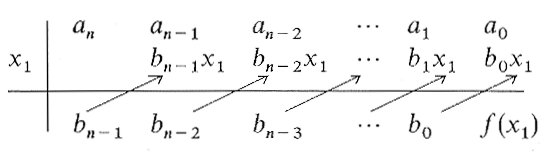
\includegraphics[width=6cm]{Content/Rechenregeln/hornerschema_1.png}\\
		$x_1 \Rightarrow$ Nullstelle (muss erraten werden!!)\\
		oberste Zeile = zu zerlegendes Polynom			
	\end{minipage}
	\begin{minipage}[t]{9cm}
		\textbf{Beispiel:}\\
		$f(x) = x^3-67x-126$\\
		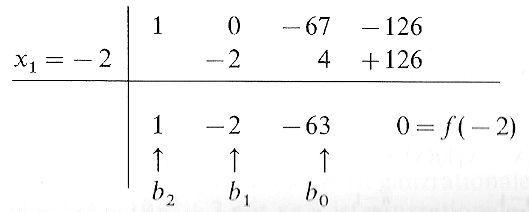
\includegraphics[width=6cm]{Content/Rechenregeln/hornerschema_2.png}\\
		$\Rightarrow f(x) = (x-x_1)(b_2x^2 + b_1x + b_0) = (x+2)(x^2-2x-63)$	
	\end{minipage}
			
	\subsection{Trigonometrie}
			$\sin^2(b)+\cos^2(b)=1 \qquad \tan(b)=\frac{\sin(b)}{\cos(b)} \qquad \cosh(b)^2 - \sinh(b)^2 = 1 \qquad \tanh(b)=\frac{\sinh(b)}{\cosh(b)}$
\subsubsection{Funktionswerte für Winkelargumente}
	\renewcommand{\arraystretch}{1.5}
	\begin{minipage}{5cm}
		\begin{tabular}[c]{ |c|c||c|c|c| }
	    	\hline
			deg & rad & sin & cos & tan\\
			\hline
			0\symbol{23} & 0 & 0 & 1 & 0\\
			\hline
			30\symbol{23} & $\frac{\pi}{6}$ & $\frac{1}{2}$ & $\frac{\sqrt{3}}{2}$ &
			$\frac{\sqrt{3}}{3}$\\
			\hline
			45\symbol{23} & $\frac{\pi}{4}$ & $\frac{\sqrt{2}}{2}$ & $\frac{\sqrt{2}}{2}$
			& 1\\
			\hline
			60\symbol{23} & $\frac{\pi}{3}$ & $\frac{\sqrt{3}}{2}$ & $\frac{1}{2}$ &
			$\sqrt{3}$\\
			\hline			
		\end{tabular}			
	\end{minipage}
	\begin{minipage}{4.3cm}
		\begin{tabular}[c]{ |c|c||c|c|}
	    	\hline
			deg & rad & sin & cos\\
			\hline
			90\symbol{23} & $\frac{\pi}{2}$ & 1 & 0\\
			\hline	
			120\symbol{23} & $\frac{2\pi}{3}$ & $\frac{\sqrt{3}}{2}$ & $-\frac{1}{2}$ \\
			\hline
			135\symbol{23} & $\frac{3\pi}{4}$ & $\frac{\sqrt{2}}{2}$ & $-\frac{\sqrt{2}}{2}$\\
			\hline
			150\symbol{23} & $\frac{5\pi}{6}$ & $\frac{1}{2}$ & $-\frac{\sqrt{3}}{2}$\\
			\hline
		\end{tabular}			
	\end{minipage}
	\begin{minipage}{4.5cm}
		\begin{tabular}[c]{ |c|c||c|c| }
	    	\hline
			deg & rad & sin & cos\\
			\hline
			180\symbol{23} & $\pi$ & 0 & -1\\
			\hline	
			210\symbol{23} & $\frac{7\pi}{6}$ & $-\frac{1}{2}$ & $-\frac{\sqrt{3}}{2}$\\
			\hline
			225\symbol{23} & $\frac{5\pi}{4}$ & $-\frac{\sqrt{2}}{2}$ & $-\frac{\sqrt{2}}{2}$\\
			\hline
			240\symbol{23} & $\frac{4\pi}{3}$ & $-\frac{\sqrt{3}}{2}$ & $-\frac{1}{2}$\\
			\hline
		\end{tabular}			
	\end{minipage}
	\begin{minipage}{4.5cm}
		\begin{tabular}[c]{ |c|c||c|c| }
	    	\hline
			deg & rad & sin & cos\\
			\hline
			270\symbol{23} & $\frac{3\pi}{2}$ & -1 & 0\\
			\hline	
			300\symbol{23} & $\frac{5\pi}{3}$ & $-\frac{\sqrt{3}}{2}$ & $\frac{1}{2}$\\
			\hline
			315\symbol{23} & $\frac{7\pi}{4}$ & $-\frac{\sqrt{2}}{2}$ & $\frac{\sqrt{2}}{2}$\\
			\hline
			330\symbol{23} & $\frac{11\pi}{6}$ & $-\frac{1}{2}$ & $\frac{\sqrt{3}}{2}$\\
			\hline
		\end{tabular}			
	\end{minipage}
	\renewcommand{\arraystretch}{1}
	
\subsubsection{Quadrantenbeziehungen}
	\begin{tabbing}
    	xxxxxxxxxxxxxxxxxxxxxxxxxxxxxxxxxx \= \kill
	  	$\sin(-a)=-\sin(a)$ \> $\cos(-a)=\cos(a)$\\
		$\sin(\pi - a)=\sin(a)$ \> $\cos(\pi - a)=-\cos(a)$\\
		$\sin(\pi + a)=-\sin(a)$ \> $\cos(\pi +a)=-\cos(a)$\\
		$\sin\left(\frac{\pi}{2}-a \right)=\sin\left(\frac{\pi}{2}+a \right)=\cos(a)$ \>
		$\cos\left(\frac{\pi}{2}-a \right)=-\cos\left(\frac{\pi}{2}+a \right)=\sin(a)$  
    \end{tabbing}

	\textbf{Additionstheoreme}
		$\sin(a \pm b)=\sin(a) \cdot \cos(b) \pm \cos(a) \cdot \sin(b) \qquad
		\cos(a \pm b)=\cos(a) \cdot \cos(b) \mp \sin(a) \cdot \sin(b)$\\ 
		$\tan(a \pm b)=\dfrac{\tan(a) \pm \tan(b)}{1 \mp \tan(a) \cdot \tan(b)}$
		
	\subsubsection{Doppel- und Halbwinkel}	
		\begin{tabular}{ll}
			$\sin(2a)=2\sin(a)\cos(a)$ &
			$\cos(2a)=\cos^2(a)-\sin^2(a)=2\cos^2(a)-1=1-2\sin^2(a)$\\
			$\cos^2 \left(\frac{a}{2}\right)=\frac{1+\cos(a)}{2}$ &
			$\sin^2 \left(\dfrac{a}{2}\right)=\frac{1-\cos(a)}{2}$
		\end{tabular}\\
		
	\begin{minipage}[t]{9.5cm}	
		\subsubsection{Produkte}
			$\sin(a)\sin(b)=\frac{1}{2}(\cos(a-b)-\cos(a+b))$\\
			$\cos(a)\cos(b)=\frac{1}{2}(\cos(a-b)+\cos(a+b))$\\
			$\sin(a)\cos(b)=\frac{1}{2}(\sin(a-b)+\sin(a+b))$
		\subsubsection{Hyperbolic}
			$\sinh(z) = \frac{1}{2} \left( e^z - e^{-z} \right) \qquad \cosh(z) =
			\frac{1}{2} \left( e^z + e^{-z} \right) $
	\end{minipage}
	\hfill
	\begin{minipage}[t]{9.5cm}		
		\subsubsection{Summe und Differenz}
			$\sin(a)+\sin(b)=2 \cdot \sin \left(\frac{a+b}{2}\right) \cdot
			\cos\left(\frac{a-b}{2}\right)$\\
			$\sin(a)-\sin(b)=2 \cdot \sin \left(\frac{a-b}{2}\right) \cdot
			\cos\left(\frac{a+b}{2}\right)$\\
			$\cos(a)+\cos(b)=2 \cdot \cos \left(\frac{a+b}{2}\right) \cdot
			\cos\left(\frac{a-b}{2}\right)$\\
			$\cos(a)-\cos(b)=-2 \cdot \sin \left(\frac{a+b}{2}\right) \cdot
			\sin\left(\frac{a-b}{2}\right)$\\
			$\tan(a) \pm \tan(b)=\dfrac{\sin(a \pm b)}{\cos(a)\cos(b)}$
	\end{minipage}	
	
		
	\subsubsection{Euler}
	$sin(z)=\frac{e^{jz}-e^{-jz}}{2j} \hspace{2cm}
    cos(z)=\frac{e^{jz}+e^{-jz}}{2} \hspace{2cm}
    e^{j\varphi}=cjs(\varphi)=cos(\varphi)+j sin(\varphi)$
    
    \subsubsection{Komplex}
    \begin{tabular}{lll}
     	Betrag: & $ |z| = \sqrt{Re(z)^2 + Im(z)^2} = \sqrt{z \cdot \bar{z}}$\\ 
     	Konjugiertkomplex: & $z=z_1 + jz_2$ & $\bar{z}=z^*=z_1-jz_2$
     \end{tabular}
	

	\subsection{Differentialrechnung}
		$f'(x_0)=\lim\limits_{\Delta x\rightarrow 0} \frac{f(x_0+\Delta) x-f(x_0)}{\Delta x}$	
		
		Kettenregel: $\frac{d f(g(x))}{dx} = f'(g(x)) \cdot g'(x)$
			
	\subsection{Taylor Polynom}
		$f(x_0+h)=f(x_0) + f'(x_0)h + \frac{f''(x_0)}{2}h^2 + \frac{f'''(x_0)}{3!}h^3 + \ldots + \frac{f^{(n)}(x_0)}{n!}h^n + R_n(x_0, h)$

	\subsection{Integralrechnung}	
	\begin{tabbing}
	     xxxxxxxxxxxxxxxxxxxxxxxxxxxxxxx \= xxx \= xxxxxxxxxxxxxxxxxxxxxxxxxxxxxxxxxxxxxxxxxxxxxxxxxxxxxxx\kill  
	     Integration\>\>$A=\int\limits_{a}^{b}{f(t)dt}=\left[F(t)\right]_a^b=F(b)-F(a)$\\[0.2cm]
	     Linearität\>		  
	   $\qquad\int{f(\alpha x+\beta )dx=\frac{1}{\alpha}\cdot F(\alpha x+
				\beta)+C}$\\[0.2cm]
		   Partielle Integration\>
	   $\qquad\int\limits_a^b{\underset{\Uparrow}{u}'(x)\cdot \underset{\Downarrow}{v}(x)dx}=\biggl[ u(x)\cdot v(x) \biggr]_a^b
	   -\int\limits_a^b{u(x)\cdot v'(x)dx}$\\[0.2cm]
	   Substitution (Rationalisierung)\>
	   $\qquad t=\tan\frac{x}{2}, \qquad dx=\frac{2dt}{1+t^2} \qquad 
	   \sin  x=\frac{2t}{1+t^2} \qquad \cos x=\frac{1-t^2}{1+t^2}
				\quad\int{R(\sin(x)\cos(x))dx}$\\ 
	   Allgemeine Substitution \> \>
				$\int\limits_{a}^{b}{f(x)dx}=\int\limits_{g^{-1}(a)}^{g^{-1}(b)}{f(g(t))\cdot
				g'(t)dt}\qquad t=g^{-1}(x)\qquad  \fbox{x=g(t)}\qquad dx=g'(t)\cdot dt$\\
	   Logarithmische Integration \>\>
	    $ \int{\frac{f'(x)}{f(x)}dx}=\ln|f(x)|+C	\qquad{(f(x)\neq 1)}$\\[0.2cm]
	  Spezielle Form des Integranden \>\>
		 		$\int{f'(x)\cdot (f(x))^{\alpha} dx}= f(x)^{\alpha +1}\cdot
		 		\frac{1}{\alpha+1}+C \qquad{(\alpha \neq -1)}$\\ 
	   Differentiation\>\>
		 		$\int \limits ^{b} _{a} {f'(t)dt}=f(b)-f(a)$\qquad
				$\frac{d}{dx} \int \limits ^{x} _{1} {f(t)dt}=f(x)$
	\end{tabbing}
	%\subsubsection{Einige unbestimmte Integrale}
	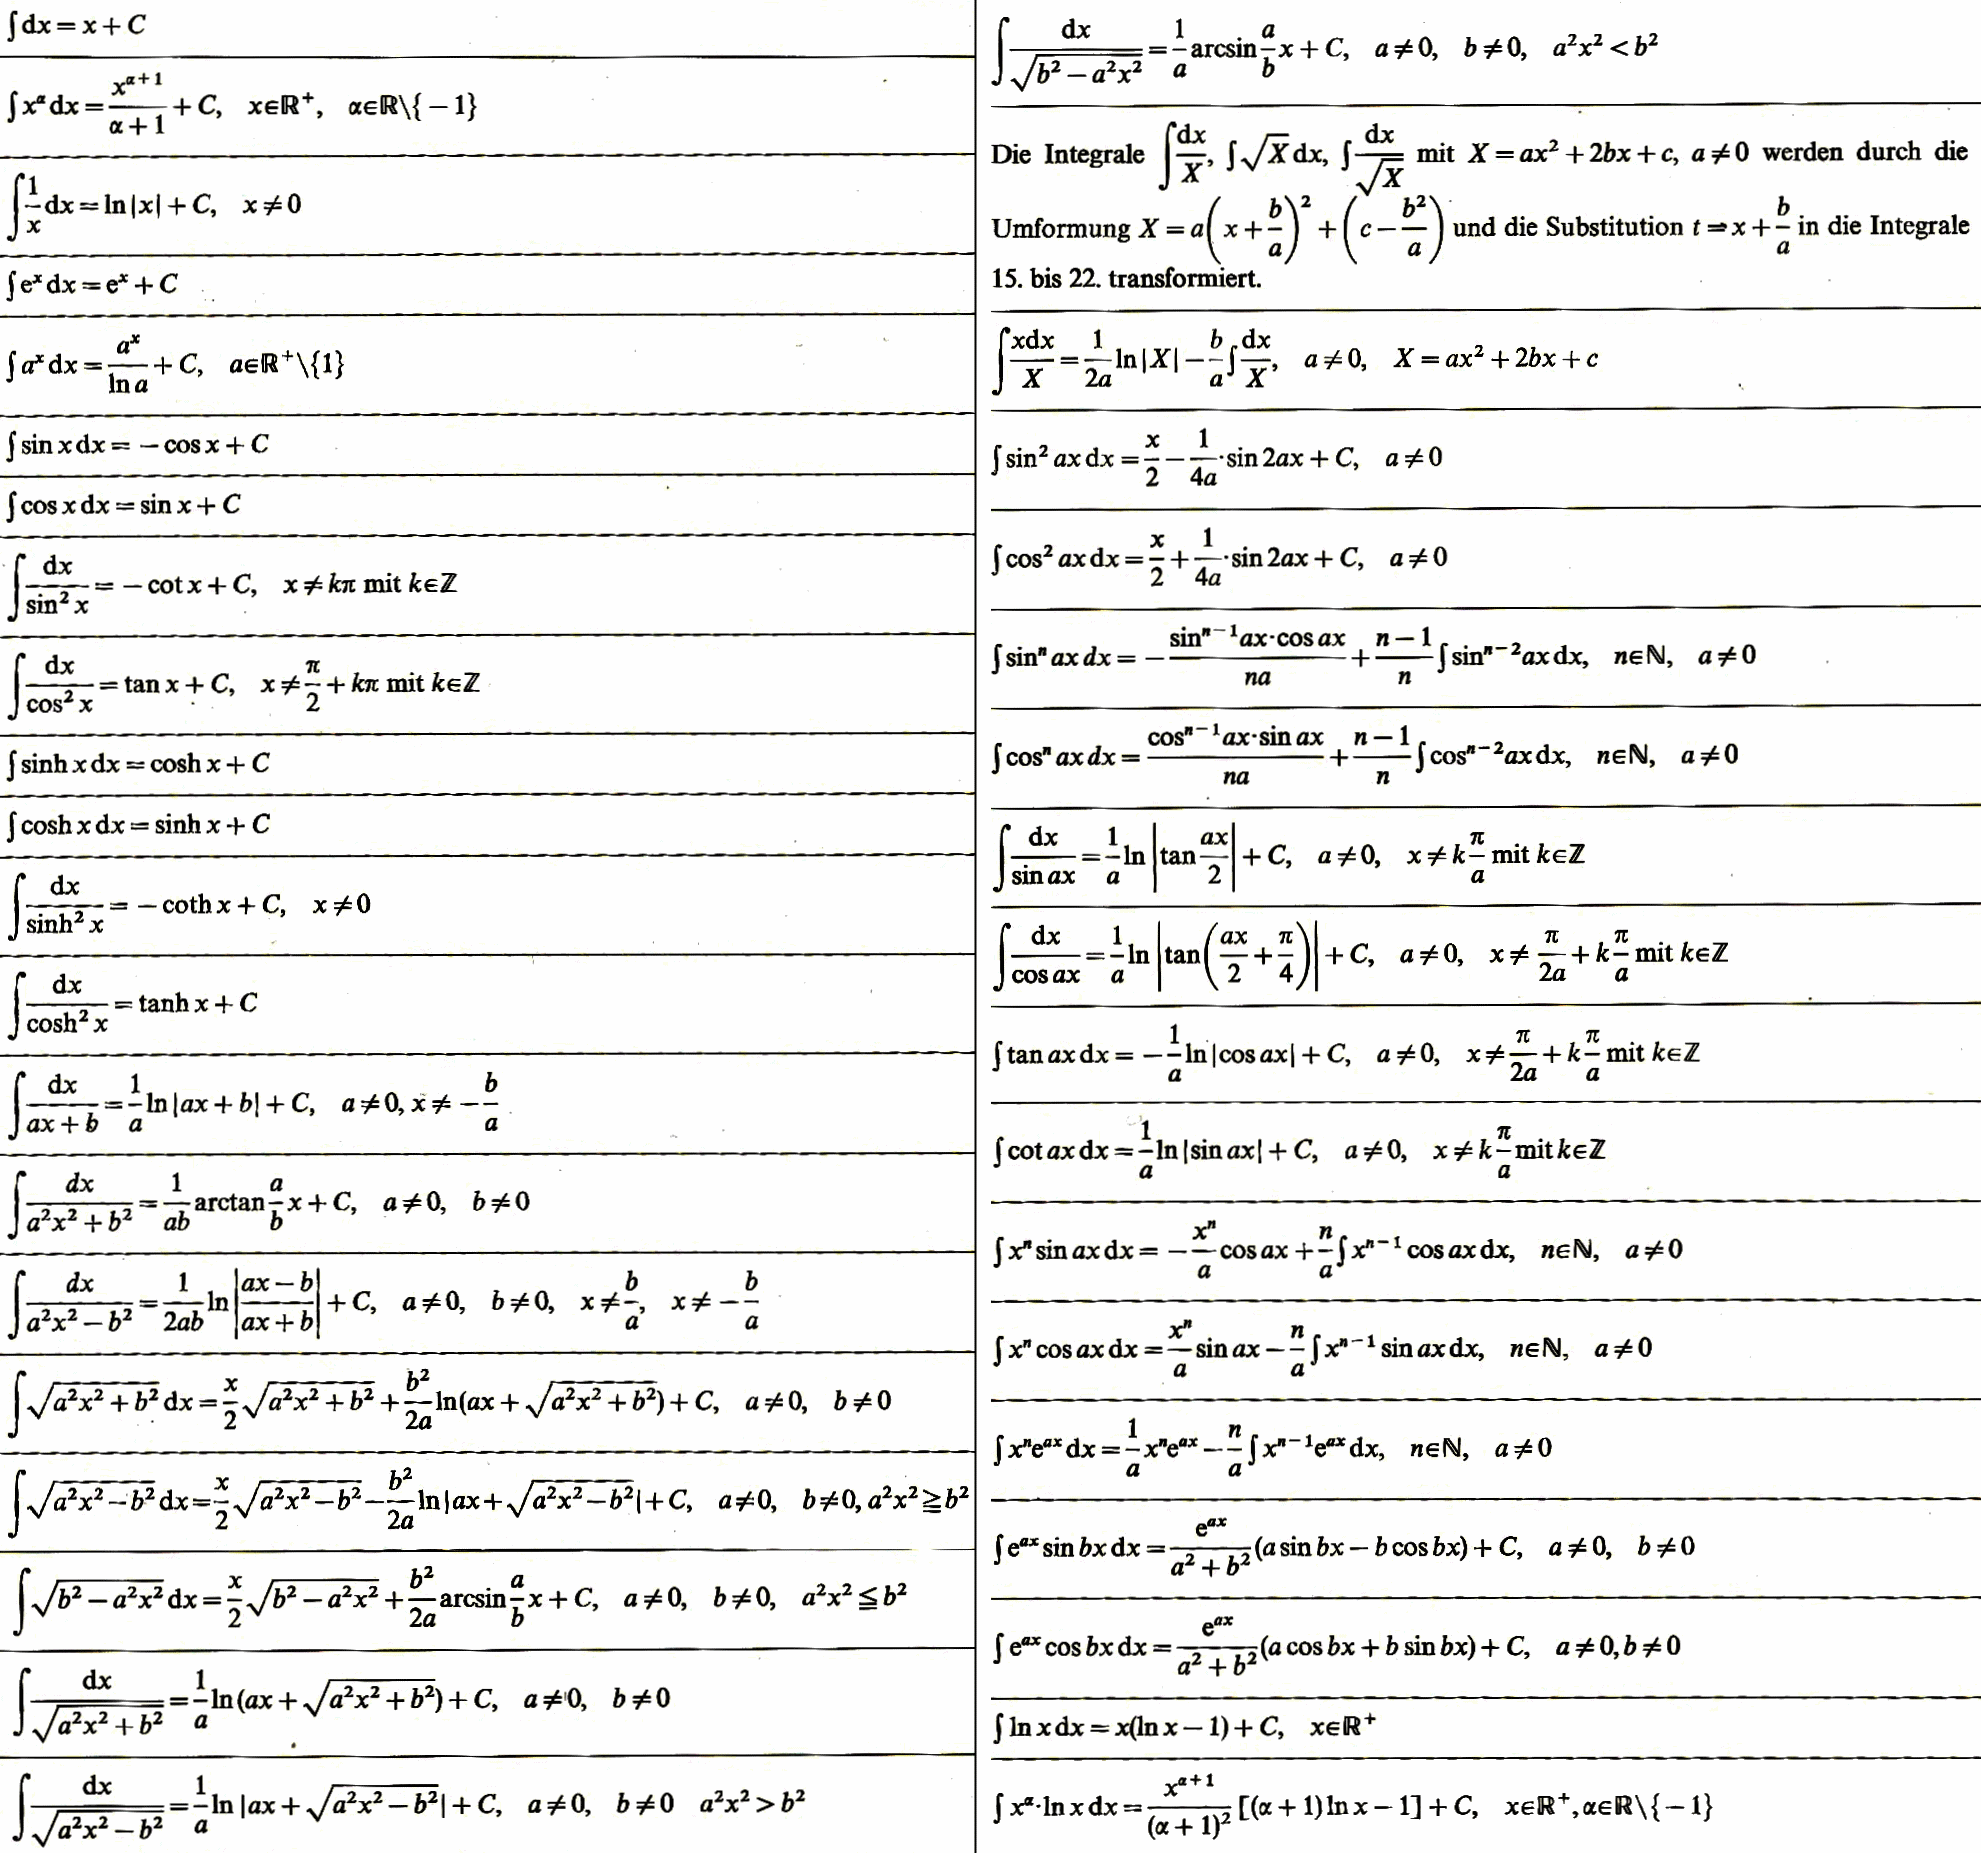
\includegraphics[width=19cm]{Content/Rechenregeln/integrale.png} 
	
	
			
	\subsection{Differentialgleichungen}
			\subsubsection{Lineare Differentialgleichungen 1. Ordnung}
	\begin{tabular}{lll}
	\textbf{Form:} $ y'+f(x)y = g(x) $ &
	\textbf{Vorgehen:} $y=y_H+y_p$ &
	$y_H=k \cdot e^{-\int f(x) dx}$ wobei $k=y_0$\\ & &
	$y_p=k \cdot e^{-\int f(x) dx}$ wobei $k=\int(g(x) \cdot e^{\int f(x) dx}) dx$
	\end{tabular}
	
	\subsubsection{Lineare Differentialgleichung 2. Ordnung mit konstanten 
	Koeffizienten}
	\begin{tabular}{p{8cm}p{8cm}}
	\textbf{Form:} $y''+a_1\cdot y'+a_0\cdot y=f(x)$  &
	\textbf{St"orglied:} $f(x)$\\
	\textbf{Homogene Differentialgleichung:} $f(x)=0$ &
	\textbf{Inhomogene Differentialgleichung:} $f(x)\neq 0$
	\end{tabular}
	
	\subsubsection{Allgemeine Lösung einer homogenen DGL:\quad\subsubadd{$\quad
	Y_H$}}
	\textbf{Charakteristisches Polynom}
	$\qquad\underline{\lambda^2+a_1\cdot\lambda+a_0=0}$ \hspace{1cm}von
	$\qquad\underline{y''+a_1\cdot y'+a_0\cdot y=0}$ 
	$\qquad(\lambda_{1,2} = -\frac{a_1}{2} \pm \frac{\sqrt{a_1^2 - 4a_0}}{2})$\\ \\
	\begin{tabular}{p{8cm}p{8cm}}
	Falls $\lambda_1\neq \lambda_2$ und $\lambda_{1,2} \in R$:&
	$Y_H=Ae^{\lambda_1x}+Be^{\lambda_2x}$\\
	Falls $\lambda_1=\lambda_2$ und $\lambda_{1,2} \in R$:    &
	$Y_H=e^{\lambda_1x}(A+B\cdot x)$\\
	Falls $\lambda_{1,2}=-\frac{a_1}{2}\pm j\alpha$:          &
	$Y_H=e^{-\frac{1}{2}a_1x}(Acos(\alpha x) +Bsin(\alpha x))$\\
	\end{tabular}\\
	
	\subsubsection{Allgemeine L"osung einer inhomogenen DGL:\quad\subsubadd{$y=Y_H+y_P$}}
	
	\textbf{Grundl"oseverfahren einer inhomogenen DGL:\quad\subsubadd{$\quad y_P$}}\\
	Homogene DGL: $y''+a_1\cdot y'+a_0\cdot y=0$  f"ur die ($g(x)=Y_H$ homogene Loesung)  $g(x_0)=0$  und
	$g'(x_0)=1$  gilt, ist:\\
	$$y_P(x)=\int\limits_{x_o}^{x} g(x+x_0-t)\cdot f(t)dt$$\\
	die partikul"are L"osung von $y''+a_1\cdot y'+a_0\cdot y=f(x)$\\
	
	\textbf{Der Ansatz einer inh. DGL in Form des
	St"orgliedes:\quad\subsubadd{$\quad y_P$}}\\
	
	 $f(x)=p_n(x)$\hspace{9cm}($p_n(x)$
	und $q_n(x)$ sind Polynome vom gleichen Grad)\\
	\begin{tabular}{p{8cm}p{4cm}}
	Fall a: $a_0\neq 0$:          & $y_P = q_n(x)$\\
	Fall b: $a_0 = 0 , a_1\neq 0$:& $y_P=x\cdot q_n(x)$\\
	Fall c: $a_0=a_1=0$:          & $y_P=x^2\cdot q_n(x)$\\
	\end{tabular}\\
	\\
	
	$f(x)=e^{bx}\cdot p_n(x)$\\
	\begin{tabular}{p{8cm}p{4cm}}
	Fall a: $b$ nicht Nullstelle des char. Polynoms:    &
	$y_P=e^{bx}\cdot q_n(x)$\\
	Fall b: $b$ einfache Nullstelle des char. Polynoms: &
	$y_P=e^{bx}\cdot x \cdot q_n(x)$\\
	Fall c: $b$ zweifache Nullstelle des char. Polynoms:&
	$y_P=e^{bx}\cdot x^2\cdot q_n(x)$\\
	\end{tabular}\\
	\\
	
	$f(x)=e^{cx}\cdot (p_n(x)\cos(bx)+q_n(x)\sin(bx))$\\
	\begin{tabular}{p{8cm}p{8cm}}
	Fall a: $c+jb$ nicht Loesung der char. Gleichung:    &
	$y_P=e^{cx}\cdot (r_n(x)\cos(bx)+s_n(x)\sin(bx))$\\
	Fall b: $c+jb$ Loesung der char. Gleichung: &
	$y_P=e^{cx}\cdot x\cdot(r_n(x)\cos(bx)+s_n(x)\sin(bx))$\\
	\end{tabular}\\
	\\

	\textbf{Superpositionsprinzip}
	
	$f(x)=c_1f_1(x)+c_2f_2(x)$\\
	\begin{tabular}{p{8cm}p{4cm}}
	$y_1$ ist spezielle L"osung der DGL &
	$y''+a_1\cdot y'+a_0\cdot y=c_1f_1(x)$ \\
	$y_2$ ist spezielle L"osung der DGL &
	$y''+a_1\cdot y'+a_0\cdot y=c_2f_2(x)$ \\
	dann ist:                          &
	$y_P=c_1y_1+c_2y_2$\\
	\end{tabular}
	
	\newpage
	
	\subsubsection{Lineare Differentialgleichung n. Ordnung mit konstanten Koeffizienten}
	\begin{tabular}{p{4cm}p{12cm}}
	\textbf{Form:} &
	$y^{(n)}+a_{n-1}\cdot y^{(n-1)}+\ldots +a_0\cdot y=f(x)$ $\Leftrightarrow$ $\sum\limits_{k=0}^na_ky^{(k)}=f(x)$\\
	\end{tabular}
	
	\textbf{Homogene L"osungen}\\
	\begin{tabular}{lll}
	Fall a: r reelle L"osungen $\lambda$: 
		& $y_1=e^{\lambda x}$, $y_2=xe^{\lambda x}$, \ldots
		,$y_r=x^{r-1}e^{\lambda x}$ 
		& Starke D"ampfung/Kriechfall\\
	Fall b: $k$ komplexe L"osungen $\lambda=\alpha +j\beta$: 
		&$y_1=e^{\alpha x}\cos(\beta x)$, $y_{3}=e^{\alpha x}x^1\cos(\beta
	x),...$ (ungerade)
		& Schwache D"ampfung /\\
		&$y_{2}=e^{\alpha x}\sin(\beta x)$, $y_{4}=e^{\alpha
	x}x^{1}\sin(\beta x),...$ (gerade)
		& Schwingfall\\
	\end{tabular}
	
	Freiheitsgrade $(A,B,C, ...)$ und zusaetzliches $x^{n}$ nicht vergessen!!! 
	
	\textbf{Allgemeinste L"osung des partikul"aren Teils:}\\
	$$\underbrace{\sum_{k=0}^n a_k y^{(k)}}_{f(y,y',y'',\ldots)} = \underbrace{e^{\alpha x} (p_{m1}(x) \cos (\beta x) + q_{m2}(x) \sin (\beta x))}_{\text{St"orglied}}$$
	Unterscheide die L"osungen des charakteristischen Polynoms ($\lambda$):\hspace{5.5cm}mit m = max(m1, m2)\\
	\begin{tabular}{p{8cm}p{8.5cm}}
	Fall a: $\alpha + j\beta \neq \lambda$, so ist &
	$y_P = e^{\alpha x}(r_m(x)\cos(\beta x) + s_m(x) \sin(\beta x))$\\
	Fall b: $\alpha + j\beta$  ist u-fache L"osung von $\lambda$, so ist &
	$y_P = e^{\alpha x} x^u (r_m(x) \cos(\beta x) + s_m(x) \sin(\beta x))$\\
	&
	u-fache Resonanz
	
	\end{tabular}
	
	\textbf{Grundl"oseverfahren}\\
	\begin{tabular}{p{12cm}p{5cm}}
	$\begin{pmatrix}
	g(x_0)=  & 0 & = & c_1g_1(x_0)+c_2g_2(x_0)+\ldots +c_n(x_0)\\
	g'(x_0)= & 0 & = & c_1g_1'(x_0)+c_2g_2'(x_0)+\ldots +c_ng_n'(x_0)\\
	\vdots  & \vdots & \\                            
	g^{(n-1)}(x_0)= & 1 & = & c_1g_1^{(n-1)}(x_0)+c_2g_2^{(n-1)}(x_0)+\ldots
	+c_ng_n^{(n-1)}(x_0)
	\end{pmatrix}$ &
	\begin{minipage}[t]{5cm}
	ergibt $c_1,\ldots ,c_n$ f"ur\\
	$y_{P}(x)=\int_{x_0}^x{g(x+x_0-t)f(t)dt}$
	\end{minipage}
	\end{tabular}
	
	
	\subsubsection{Lineare Differentialgleichungssysteme erster Ordnung mit konstanten
	Koeffizienten}
	\begin{tabular}{p{8cm}p{8cm}}
	\textbf{Form:}&
	$\dot{x}=ax+by+f(t) \leftrightarrow y=\frac{1}{b}(\dot{x}-ax-f(t))$\\
	&
	$\dot{y}=cx+dy+g(t)$\\
	\textbf{Die allgem. L"osung ergibt sich aus der DGL:}&
	$\ddot{x}-(a+d)\dot{x}+(ad-bc)x=\dot{f}(t)-d \cdot f(t)+b \cdot g(t)$\\
	\end{tabular}
	
	$\ddot{x}, \dot{x}, \dot{y}$ sind jeweils nach $t$ abgeleitet!
	
	\subsubsection{DGL mit Laplacetransformation L"osen}
		Um eine DGL mit Laplace(kausal!) zu l"osen muss die gleichung zuerst in den
		Bildbereich transformiert werden. Nachher kann die gleichung Algebraisch
		gel"ost werden. Das Resultat muss dann "uber die R"ucktransformation wieder in
		den Orginalbereich transformiert werden.  \\
	
		Bemerkung:\\
		- $H(s)=\frac{1}{p(s)}$ wobei $p(s)$ das charakteristische Polynom darstellt

		\textbf{Stabilit"at}\\
			Ein System ist Stabil wenn die Nullstelle vom charakteristischen Polynom
			$p(s)$ in der Linken Halbebene zuliegen kommt:\\
			$$Re[p(s)] < 0$$
			
	\subsubsection{G"angige DGLs}
	  \label{sec:dgls}
	  \begin{tabular}{ll | ll}
	    DGL & L"osung & DGL & L"osung\\[0.2cm]
      $\dfrac{dx}{dt} =0$
      & $x_0$
 	    & $\dfrac{dx}{dt} =1$
 	    & $t + x_0$\\[0.2cm]
	    $\dfrac{dx}{dt} = y$
	    & $y \cdot t$
	    & $\dfrac{dx}{dt} = x$
	    & $C e^{t}$\\[0.2cm]
	    $\dfrac{d u}{dt} = \sin(u)$
	    & $- \cos(u)$
	    & $\dfrac{d^2 x}{dt^2} = x$
	    & $\sinh(t)$ oder $\cosh(t)$\\[0.2cm]
	    $\dfrac{d^2 x(t)}{dt^2} = -\omega^2 x(t)$
	    & $A \omega \cos(\omega t) - B \omega \sin(\omega t)$
	    & & 
	  \end{tabular}
	
	\subsection{Divers}	
	\begin{minipage}[t]{9.5cm}
		\subsubsection{Quadratische L�sungsformel}
			$ax^2+bx+c=0\quad\Rightarrow\quad x_{1,2}=\frac{-b\pm\sqrt{b^2-4ac}}{2a}$
	\end{minipage}
	\hfill
	\begin{minipage}[t]{9.5cm}
		\subsubsection{Determinanten}
			$\det\left(
			\begin{bmatrix}
				a_{11}&a_{12}\\
				a_{21}&a_{22}\\
			\end{bmatrix}\right)=
			\begin{vmatrix}
				a_{11}&a_{12}\\
				a_{21}&a_{22}\\
			\end{vmatrix}=a_{11}a_{22}-a_{12}a_{21}$
	\end{minipage}\\
	
	
	\begin{minipage}[t]{9.5cm}
		\subsubsection{Matrizeninversion}
			$A=\begin{bmatrix}
						a_{11}&a_{12}\\
						a_{21}&a_{22}\\
				\end{bmatrix}\quad\Rightarrow\quad
			A^{-1}=\frac{1}{det(A)}
			\begin{bmatrix}
				a_{22}&-a_{12}\\
				-a_{21}&a_{11}\\
			\end{bmatrix}$
	\end{minipage}
	\hfill
	\begin{minipage}[t]{9.5cm}
		\subsubsection{Eigenwerte/ Eigenvektoren}
			Eigenwert: $\det(A-\lambda I)\quad\Rightarrow\quad \lambda i$\\
			Eigenvektor: $(A-\lambda_i I)v=0\quad\Rightarrow\quad v_i\qquad(\text{F�r jedes }\lambda_i)$
	\end{minipage}
	
